%%%%%%%%%%%%%%%%%%%%%%%%%%%%%%%%%%%%%%%%%%%%%%%%%%%%%%%%%%
%%
%%  LOD-L6.tex
%%  Lecture 6: Diffeology Fiber Bundles
%%
%%%%%%%%%%%%%%%%%%%%%%%%%%%%%%%%%%%%%%%%%%%%%%%%%%%%%%%%%%

\chapter*{\S L6. Diffeology Fiber Bundles}
\setcounter{footnote}{0}

%%%%%%%%%%%%%%%%%%%%%%%%%%%%%%%%%%%%%%%%%%%%%%%%%%%%%%%%%%
%%
%% MARK: Abstract
%%
%%%%%%%%%%%%%%%%%%%%%%%%%%%%%%%%%%%%%%%%%%%%%%%%%%%%%%%%%%
\begin{abstract}
  This lecture talks about the theory of diffeology fiber bundles,
  which deviates from the usual locally trivial bundles,
  where local triviality is replaced in diffeology by local triviality along the plots.
  We illustrate this definition with a few examples where some new situations happen only in diffeology.
\end{abstract}

%%%%%%%%%%%%%%%%%%%%%%%%%%%%%%%%%%%%%%%%%%%%%%%%%%%%%%%%%%
%%
%% MARK: Introduction
%%
%%%%%%%%%%%%%%%%%%%%%%%%%%%%%%%%%%%%%%%%%%%%%%%%%%%%%%%%%%

The question of what is a fiber bundle in diffeology arises immediately with the case of irrational torus $\Torus_\alpha$.
A direct computation of the first homotopy group shows that the projection $\Torus^2 \to  {\Torus}_{\alpha}$ behaves like a fibration,
with fiber $\RR$,
but without being locally trivial,
since ${\Torus}_{\alpha}$ inherits the coarse topology.
Indeed,
from the diffeology we found directly that
$$%
  \pi_0(\Torus_\alpha) = \{\Torus_\alpha\}
  \SpacedText{and}
  \tilde{T}_\alpha = \RR
  \SpacedText{with}
  \pi_1(\Torus_\alpha) = \ZZ + \alpha \ZZ \subset \RR,
$$%
where $\tilde{T}_\alpha$ plays the role of \emph{universal covering} of $\Torus_\alpha$.

So,
it was necessary to revise the notion of fiber bundle from classical differential geometry,
and adapt it to diffeology in order to include these new objects,
specific to diffeology,
but without losing the main properties of this theory.
This is what I have done in my ScD dissertation in 1985 \cite{Igl85}.

The main properties we wanted to preserve were:

\begin{enumerate}
  \item The homotopy long sequence,
  that we shall see in the lecture on homotopy.
  \item Any quotient $\Class \colon G \to G/H$ is a diffeological fiber bundle,
  with fiber $H$,
  where $G$ is a diffeological group and $H$ any subgroup.
\end{enumerate}

These two properties,
if satisfied,
will explain the direct calculation of the homotopy of the irrational torus we did in \cite{DI83}.

In this lecture we shall see two equivalent definitions of \emph{diffeological fiber bundles}.
The first is pedestrian and operative,
involving \emph{local triviality along the plots}.
The second one involving groupoids is more in the spirit of diffeology.

%%%%%%%%%%%%%%%%%%%%%%%%%%%%%%%%%%%%%%%%%%%%%%%%%%%%%%%%%%
%%
%% MARK:  Diffeological Fiber Bundles, the Pedestrian Approach
%%
%%%%%%%%%%%%%%%%%%%%%%%%%%%%%%%%%%%%%%%%%%%%%%%%%%%%%%%%%%
\section{Diffeological fiber bundles, the pedestrian approach}

\begin{Article}{Category of projections.}{}
  We call \emph{projection} any smooth surjection $\pi \colon Y \to X$,
  with $X$ and $Y$ two diffeological spaces.
  The space $Y$ is called the \emph{total space} of the projection and $X$ is called the \emph{base}.
  We define a category \{Projections\} whose objects are the projections and:

  \uline{Definition 1.} {\itshape The \emph{morphisms}
  from $\pi \colon Y \to X$  to $\pi' \colon Y' \to X'$,
  are the pairs of smooth maps $(\Phi,\pphi)$ such that:
  $$%
    \Phi \in \Cinfty(Y,Y')
    \SpacedText{and}
    \pphi \in \Cinfty(X,X'),
  $$%
  such that
  $$%
    \begin{tikzcd}[column sep=2em, row sep=2em,every label/.append style = {font = \small}]
    Y \arrow[d, swap, "\pi"]  \arrow[r, "\Phi"] &  Y' \arrow[d,"\pi'"] \\
    X \arrow[r, swap, "\pphi"] & X'
    \end{tikzcd}
    \SpacedText{with}
    \pi' \circ \Phi = \pphi \circ \pi.
  $$%
  }
  The preimage
  $$%
    \pi^{-1}(x) = \{y \in Y \mid \pi(y) = x\}
  $$%
  is called the \emph{fiber} of the projection over $x$.
  I use also the word \emph{bundle} as synonym of projection,
  which will be specified in some cases in fiber bundle later,
  when some other properties will be satisfied.

  \uline{Definition 2.} {\itshape An \emph{isomorphism} from $\pi$ to $\pi'$ will be a pair $(\Phi,\pphi)$ of diffeomorphisms.}
\end{Article}

\begin{Article}{Pullbacks of bundles.}{}
  Let $\pi \colon Y \to X$ be a projection.
  Let $f \colon X' \to X$ be a smooth map.
  We call \emph{the total space of the pullback} of $\pi$ by $f$,
  or simply the \emph{pullback},
  the space denoted and defined by
  $$%
    f^*(Y) = \{ (x',y) \in X' \times Y \mid f(x) = \pi(y) \}.
  $$%
  This set is equipped with the subset diffeology of the product $X' \times Y$.
  %
  \begin{center}
    \begin{tikzcd}[column sep=1cm, row sep=1cm,every label/.append style = {font = \small}]
      f^*(Y) \arrow[d, swap, "\Proj_1"]  \arrow[r, "\Proj_2"] &  Y \arrow[d,"\pi"] \\
      X' \arrow[r, swap, "f"] & X
    \end{tikzcd}
  \end{center}
  %
  The pullback of $\pi$ by $f$ is the first projection:
  $$%
    \Proj_1 \colon f^*(Y) \to X'
    \SpacedText{with}
    \Proj_1(x',y) = x'.
  $$%
\end{Article}

\begin{Article}{Trivial projections.}{}
  Projections on factors are particular cases of projections.
  We will see often the first projection of direct products:
  $$%
    \Proj_1 \colon X \times F \to X
  $$%
  \uline{Definition.} {\itshape We say that a projection $\pi \colon Y \to X$ is \emph{trivial with fiber $F$} if it is isomorphic to the first projection $\Proj_1 \colon X \times F \to X$.}

  It is equivalent to say that there exists an isomorphism with the first projection $\Proj_1 \colon X \times F \to X$ with type $(\Phi,\Id_X)$.
  %
  \begin{center}
    \begin{tikzcd}[column sep=2em, row sep=2em,every label/.append style = {font = \small}]
      X \times F \arrow[dr, swap, "\Proj_1"]  \arrow[rr, "\Phi"] & & Y \arrow[dl,"\pi"]  \\
      & X &
    \end{tikzcd}
  \end{center}
  %
  And that is the way we will use it in general.
\end{Article}

\begin{proof}
  Assume that $(\Phi, \pphi)$ is an isomorphism from $\Proj_1 \colon X \times F \to X$ to $\pi \colon Y \to X$.
  Consider then the isomorphism $(\pphi^{-1} \times \Id_F,\pphi^{-1})$ from $\Proj_1 \colon X \times F \to X$ to itself,
  we get:
  %
  \begin{center}
    \begin{tikzcd}[column sep=4em, row sep=2em,every label/.append style = {font = \small}]
      X \times F \arrow[d, swap, "\Proj_1"]  \arrow[r, "\pphi^{-1} \times \Id_F"] & X \times F \arrow[d, swap, "\Proj_1"] \arrow[r,"\Phi"] &  Y \arrow[d,"\pi"]  \\
      X \arrow[r, swap, "\pphi^{-1}"] &  X \arrow[r, swap, "\pphi"] & X
    \end{tikzcd}
  \end{center}
  %
  which gives
  \begin{center}
    \begin{tikzcd}[column sep=4em, row sep=2em,every label/.append style = {font = \small}]
      (x,y) \arrow[d, swap, "\Proj_1"]  \arrow[r, "\pphi^{-1} \times \Id_F"] & (\pphi^{-1}(x),y) \arrow[d, swap, "\Proj_1"] \arrow[r,"\Phi"] &  \Phi(\pphi^{-1}(x),y) \arrow[d,"\pi"]  \\
      x \arrow[r, swap, "\pphi^{-1}"] &  \pphi^{-1}(x) \arrow[r, swap, "\pphi"] & \pphi(\pphi^{-1}(x)) = x
    \end{tikzcd}
  \end{center}
  And that is the triangle diagram above.
\end{proof}

\begin{Article}{Locally trivial projections.}{}
  With trivial projection comes \emph{locally trivial} projection.
  Let $\pi \colon Y \to X$ a smooth projection as it is defined above.

  \uline{Definition.} {\itshape We say that the projection $\pi$ is \emph{locally trivial} if there exists a diffeological space $F$,
  a D-open covering $(U_i)_{i \in \cI}$ of $X$ such that the restrictions
  $$%
    \pi_i \colon Y_i \to U_i
    \SpacedText{with}
    Y_i = \pi^{-1}(U_i)
    \SpacedText{and}
    \pi_i = \pi \restriction Y_i,
  $$%
  are trivial with fiber $F$.
  }

  It is equivalent to say that:
  \begin{enumerate}
    %
    \item $\pi$ is \emph{locally trivial at the point $x \in X$},
    if there exists a D-open neighborhood $U$ of $x$ such that:
    the restriction $\pi_U \colon Y_U \to U$ is trivial,
    with $Y_U = \pi^{-1}(U)$ and $\pi_U = \pi \restriction Y_U$.
    %
    \item $\pi$ is \emph{locally trivial everywhere} with fiber $F$.
    %
  \end{enumerate}
\end{Article}

\begin{Article}{Diffeological fiber bundles.}{}
  \label{Diffeological-Fiber-Bundles}
  A smooth projection $\pi \colon Y \to X$,
  is a \emph{diffeological fibration},
  or a \emph{diffeological fiber bundle},
  if it is {\em locally trivial along the plots},
  that is,
  if the pullback of $\pi$ by any plot $P$ of $X$ is locally trivial with some given fiber $F$.
  The space $F$ is the \emph{fiber} of the fibration.

  That means precisely the following:

  For all plots $P \colon U \to X$,
  for all $r \in U$,
  there exists an open neighborhood $V$ of $r$ in $U$ such that $\Proj_1 \colon (P \restriction V)^*(Y) \to V$ is trivial with fiber $F$,
  that is,
  isomorphic to $\Proj_1 \colon V \times F \to V$.
  Recall that
  $$%
    P^*(Y) = \{ (r,y) \in U \times Y \mid P(r) = \pi(y) \}.
  $$%

  \Note{1.} A diffeological fibration $\pi \colon Y \to X$ is,
  in particular,
  a subduction and even a \emph{local subduction}.
  That is,
  for every plot $P \colon U \to X$,
  for all $r \in U$ and for all $y \in Y_x = \pi^{-1}(x)$,
  with $x = P(r)$,
  there exists a plot $Q$ of $Y$ defined on some open neighborhood $V$ of $r$ lifting $P \restriction V$,
  that is,
  $P \restriction V = \pi \circ Q$,
  and such that $Q(r) = y$.

  \Note{2.}  There is a hierarchy in the various notions of fiber bundles:

  \begin{enumerate}
    %
    \item Trivial fiber bundles are locally trivial (with respect to the D-topology).
    %
    \item Locally trivial fiber bundles are locally trivial along the plots.
    The converse is not true.
    %
  \end{enumerate}

  To be locally trivial along the plots does not mean that the fibration
  itself is locally trivial,
  as many examples will point out.
  For example,
  the projection of $\Torus^2$ on the irrational torus $\Torus_\alpha = \Torus^2/\cS_\alpha$ is locally trivial along the plots,
  with fiber $\RR$,
  but not trivial.
  This is a particular case of quotient $G/H$ of diffeological groups by a subgroup.

  \Note{3.} If the base of a diffeological fiber bundle is a manifold,
  then the fiber bundle is locally trivial.
  This comes immediately from the definition,
  consider the pullback by local charts.
  If moreover the fiber is a manifold,
  then the diffeological fiber bundle is a fiber bundle in the category of manifolds.
  This shows in particular that the classical notion of fiber bundle can also be defined directly in diffeological
  terms as a property of its associated groupoid, as we shall see later,
  but of course this definition leads to leave an instant the category of manifolds.
\end{Article}

\begin{Article}{Quotient of groups by subgroups.}{}
  Let $G$ be a diffeological group and $H \subset G$ be a subgroup.
  Then,
  the projection $\Class \colon G \to G/H$ is a diffeological fibration,
  where $H$ acts on $G$ by left multiplication denoted by $L(h)(g) = hg$.

  \Note{1.} We recall that a diffeological group is a group equipped with a diffeology such that the multiplication $(g,g') \mapsto gg'$ and the inversion $g \mapsto g^{-1}$ are smooth.

  \Note{2.} In particular the projection $\Class \colon \Torus^2 \to \Torus_\alpha = \Torus^2/\cS_\alpha$ is a diffeological fibration.
\end{Article}

\begin{proof}
  Let $P \colon U \to G/H$ be a plot.
  We have:
  $$%
    P^*(G) = \{(r,g) \in U \times G \mid \Class(g) = P(r) \}.
  $$%
  Let $r_0 \in U$,
  there exists an open neighborhood $V$ of $r_0$ and a smooth lifting of $P$,
  $Q \colon r \mapsto g_r$,
  over $V$ such that $\Class(g_r) = P(r)$.
  Let
  $$%
    \psi \colon V \times H \to (P \restriction V)^*(G)
    \SpacedText{defined by}
    \psi(r,h) = (r,hg_r).
  $$%
  The inverse is given by
  $$%
    \psi^{-1} \colon (r,g) \mapsto (r,gg_r^{-1}).
  $$%
  Since the multiplication and the inversion are smooth,
  $\psi$ and $\psi^{-1}$ are smooth and $\psi$ is an isomorphism from $V \times H$ to $(P \restriction V)^*(G)$,
  for $\Proj_1$ both sides.
  Therefore $\Class \colon G \to G/H$ is a diffeological fibration.
\end{proof}

\begin{Article}{Principal fiber bundles.}{}
  Let $X$ be a diffeological space and $g \mapsto g_X$ be a smooth action of a diffeological group $G$ on $X$,
  that is,
  a smooth homomorphism from $G$ to $\Diff(X)$ equipped with the functional diffeology of diffeological group.

  Let $\cE$ be the {\em action map},
  $$%
    \cE : X \times G \to X \times X
    \SpacedText{with}
    \cE(x,g) = (x,g_X(x)).
  $$%

  \smuline{Proposition.} {\itshape If $\cE$ is an induction,
  then the projection $\Class$ from $X$ to its quotient $X/G$ is a diffeological fibration,
  with the group $G$ as fiber.
  We shall say that the action of $G$ on $X$ is \emph{principal}.}

  \uline{Definition.} {\itshape If a projection $\pi : X \to Q$ is equivalent to $\Class : X \to G/H$,
  %
  \begin{center}
    \begin{tikzcd}[column sep=2em, row sep=2em,every label/.append style = {font = \small}]
      & X \arrow[dl, swap, "\Class"]  \arrow[dr, "\pi"] &   \\
      X/G \arrow[rr, swap, "\pphi"] &  & Q
    \end{tikzcd}
  \end{center}
  %
  that is,
  if there exists a diffeomorphism $\pphi : G/H \to Q$ such that $\pi = \pphi \circ \Class$,
  then we shall say that $\pi$ is a \emph{principal fibration},
  or a \emph{principal fiber bundle},
  with structure group $G$.}

  \Note{a)} If the action $\cE$ is inductive,
  then it is in particular injective,
  which implies that the action of $G$ on $X$ is free,
  which is indeed a necessary condition.

  \Note{b)} The quotients $\Class \colon G \to G/H$ are principal bundles with group $H$.

  \Note{c)} Let $\pi \colon X \to Q$ the $G$-principal fiber bundle,
  then the pullback of $\pi$ by any plot $P \colon U \to Q$ is locally trivial,
  let say with $\Phi \colon V \times G \to (P \restriction V)^*(X)$
  %
  \begin{center}
    \begin{tikzcd}[column sep=2em, row sep=2em,every label/.append style = {font = \small}]
      V \times G \arrow[dr, swap, "\Proj_1"]  \arrow[rr, "\Phi"] & & (P \restriction V)^*(X) \arrow[dl,"\Proj_1"]  \\
      & V &
    \end{tikzcd}
  \end{center}
  %
  and write
  $$%
    \Phi(r,g) = (r, \Phi_r(g)).
  $$%
  Then,
  the isomorphism $\Phi$ satisfies the equivariant property:
  $$%
    \Phi_r(gg') = g_X(\Phi_r(g')).
  $$%
  In particular,
  $$%
    \Phi_r(g) = g_X(\pphi(r))
    \SpacedText{with}
    \pphi(r) = \Phi_r(\Id_G).
  $$%
  And $\pphi$ is a local lifting of the plot $P$
  $$%
    \pphi \colon V \to X
    \SpacedText{and}
    \pi \circ \pphi = P \restriction V.
  $$%
  %
  \begin{center}
    \begin{tikzcd}[column sep=3em, row sep=3em,every label/.append style = {font = \small}]
      & & X \arrow[d,"\pi"]  \\
      V \arrow[r, hookrightarrow] \arrow[rru,"\pphi"] & U \arrow[r,"P"] & Q
    \end{tikzcd}
  \end{center}

  \Note{d)} A principal fiber bundle is trivial if and only if it admits a global smooth section.
\end{Article}

%%%%%%%%%%%%%%%%%%%%%%%%%%%%%%%%%%%%%%%%%%%%%%%%%%%%%%%%%%
%%
%% MARK:  Diffeological Fiber Bundles, the Groupoid Approach
%%
%%%%%%%%%%%%%%%%%%%%%%%%%%%%%%%%%%%%%%%%%%%%%%%%%%%%%%%%%%
\section{Diffeological fiber bundles, the groupoid approach}

\begin{Article}{Structure groupoid of a projection.}{}
  Let $\pi \colon Y \to X$ be a smooth surjection.
  Let us define
  $$%
    \Obj(\KK) = X \text{ and for all $x, x' \in X$, } \Mor_{\KK}(x,x') = \Diff(Y_x, Y_{x'}),
  $$%
  where the $Y_x = \pi^{-1}(x)$,
  $x \in X$,
  are equipped with the subset diffeology.
  Let us define  on
  $$%
    \Mor(\KK) = \bigcup_{x,x'\in X} \Mor_{\KK}(x,x')
  $$%
  the natural multiplication $f \cdot g = g \circ f$,
  for $f \in \Mor_{\KK}(x,x')$ and $g \in \Mor_{\KK}(x',x'')$,
  %%###########
  \begin{figure}[htb]
    \centerline{
\includegraphics[width=.65\textwidth]{Figures/fig-groupoid-projection.pdf}}
    \caption{The groupoid associated with a projection.}
    \label{groupoid-projection}
  \end{figure} %% The groupoid associated with a projection
  %%###########
  $\KK$ is clearly a groupoid.
  The source and target maps are given by
  $$%
    \Src(f) = \pi(\Def(f))
    \SpacedText{and}
    \Trg(f) = \pi(\Val(f)).
  $$%
  The groupoid $\KK$ is then equipped with a functional diffeology of $\KK$ defined as follows.
  Let $Y_\Src$ be the total space of the pullback of $\pi$ by $\Src$,
  that is,
  $$%
    Y_\Src = \{(f,x) \in \Mor(\KK) \times Y \mid x \in \Def(f) \}.
  $$%
  We define the evaluation map $\Eval$ as usual:
  $$%
    \Eval : Y_\Src \to Y
    \SpacedText{with}
    \Eval(f,x) = f(x).
  $$%
  There exists a coarsest diffeology on $\Mor(\KK)$,
  which gives to $\KK$ the structure of a diffeological groupoid and such that the evaluation map  $\Eval$ is smooth.
  It will be called again the {\em functional diffeology}.
  Equipped with this functional diffeology,
  the groupoid $\KK$ captures the {\em smooth structure} of the projection $\pi$.
  It is why we define $\KK$ as the \emph{structure groupoid} of the surjection $\pi$.

  \Note{1.} If $X$ is reduced to a point,
  $\Obj(\KK) = \{\star\}$,
  this diffeology coincides with the usual functional diffeology of $\Diff(Y) = \Mor(\KK)$.

  \Note{2.} This construction also applies when we have just a partition $\cP$ on a diffeological space $Y$.
  We can equip the quotient $Q = Y/\cP$ with the quotient diffeology,
  and we get the structure groupoid of the partition as the structure groupoid of the projection $\pi : Y \to Q$.
\end{Article}

\begin{Article}{Fibrating groupoid.}{}
  Let $\pi \colon Y \to X$ be a smooth projection.

  The projection $\pi$ is a \emph{diffeological fibration} if the structure groupoid $\KK$ is
  \emph{fibrating},
  that is,
  if and only if the characteristic map
  $$%
    \chi \colon \Mor(\KK) \to B \times B
  $$%
  is a subduction.
  In particular,
  the preimages $Y_x = \pi^{-1}(x)$,
  are necessarily all diffeomorphic since $\chi$ is surjective.

  This definition is completely equivalent to the previous one \textsection\,\ref{Diffeological-Fiber-Bundles}.
\end{Article}

%%%%%%%%%%%%%%%%%%%%%%%%%%%%%%%%%%%%%%%%%%%%%%%%%%%%%%%%%%
%%
%% MARK:  Associated Fiber Bundles
%%
%%%%%%%%%%%%%%%%%%%%%%%%%%%%%%%%%%%%%%%%%%%%%%%%%%%%%%%%%%
\section{Associated fiber bundles}

\begin{Article}{Associated fiber bundles.}{}
  Consider a principal fiber bundle  $\pi \colon Y \to X$ with group $G$.
  Let $E$ be a diffeological space with a smooth action of $G$,
  that is a smooth morphism $g \mapsto g_E$ from $G$ to $\Diff(E)$.
  Let the product over $X$ be the quotient space
  $$%
    Y \times_G E = (Y \times E)/G,
  $$%
  where $G$ acts on the product diagonally
  $$%
    g_{Y \times E}(y,e) = (g_Y(y),g_E(e)).
  $$%
  Then,
  the projection:
  $$%
    \Proj \big(\Class(y,e)\big) = \pi(y),
  $$%
  from $Y \times_G E$ to $X$ is a diffeological fiber bundle with fiber $E$.
  %
  \begin{center}
    \begin{tikzcd}[column sep=3em, row sep=3em,every label/.append style = {font = \small}]
      Y \times E \arrow[d, swap, "\Proj_1"] \arrow[r,"\Class"]  & Y \times_{G} E \arrow[d,"\Proj"]  \\
      Y \arrow[r, swap, "\pi"] & X
    \end{tikzcd}
  \end{center}
  %
\end{Article}

\begin{Article}{Main theorem.}{}
  Let $\pi \colon Y \to X$ be a diffeological fiber bundle with fiber $E$,
  then there exists a principal fiber bundle $\Proj \colon \Torus \to X$ with some diffeological group $G$ acting smoothly on $E$,
  such that $\pi$ is associated with $\Proj$.
  Actually,
  one can always take $G = \Diff(E)$.
\end{Article}

%%%%%%%%%%%%%%%%%%%%%%%%%%%%%%%%%%%%%%%%%%%%%%%%%%%%%%%%%%
%%
%% MARK:  Covering Diffeological Spaces
%%
%%%%%%%%%%%%%%%%%%%%%%%%%%%%%%%%%%%%%%%%%%%%%%%%%%%%%%%%%%
\section{Covering diffeological spaces}

A special case of fiber bundle plays a special role in differential geometry,
the covering spaces.

\begin{Article}{Covering spaces.}{}
  Let $X$ be a \emph{connected} space,
  that is,
  for all pairs of points $x,x' \in X$,
  there exists a \emph{smooth path} $\gamma \in \Paths(X) = \Cinfty(\RR, X)$ such that $\gamma(0) = x$ and $\gamma(1) = x'$.
  We say that $x$ and $x'$ are connected.

  We call \emph{covering} over $X$ any fiber bundle such that the fiber is discrete (of course diffeologically).
  The covering may be non connected but we focus in general on connected coverings.

  The main theorem about covering is about the universal covering.
\end{Article}

\begin{Article}{Universal covering.}{}
  Let $X$ be a connected diffeological space,
  there exists a unique,
  up to equivalence,
  simply connected which is a principal fiber bundle whose group is the first group of homotopy $\pi_1(X)$.
  Any other connected covering is a quotient of this one.

  Simple connectivity will be defined in the next lecture.
\end{Article}

\begin{Article}{Monodromy theorem.}{}
  Let $f \colon Y \to X$ with $X$ connected and $Y$ simply connected.
  There exists always a smooth lifting $\tilde f \colon Y \to \tilde X$ ,
  where $\pi \colon \tilde X \to X$ is the universal covering.
  That is,
  $\pi \circ \tilde f = f$.
  And if we fix three points $y \in Y$,
  $x \in X,
  \tilde x \in \tilde X$,
  such that $f(y) = x$,
  $\pi(\tilde x) = x$,
  there exists a unique lifting such that $\tilde f(y) = \tilde x$.
\end{Article}

\begin{Article}{Example: The irrational tori.}{}
  If we call irrational tori any quotient $\cQ$ of $\RR^n$ by a discrete subgroup $\Gamma$ that spans $\RR^n$,
  that is,
  $\Gamma \otimes \RR = \RR^n$,
  then $\RR^n$ is the universal covering and $\pi_1(\cQ) = \Gamma$.
\end{Article}

\begin{Article}{Example: $\bf \text{Diff}\,(\Sph^1)$.}{}
  The universal covering of group of diffeomorphisms $\Diff(\Sph^1)$ is naturally identified as
  $$%
    \widetilde\Diff(\Sph^1) \simeq \{ \tilde f \in \Diff(\RR) \mid \tilde f(x+1) = \tilde f(x) + 1 \}
  $$%
  Any $\tilde f \in \widetilde\Diff(\Sph^1)$ descends on $\Sph^1 \simeq \RR/2 \pi \ZZ$ by
  $$%
    f(\Class(x)) = \Class(f(x)),
    \SpacedText{or}
    f(e^{2i\pi x}) = e^{2 i \pi \tilde f(x)}.
  $$%
\end{Article}

%%%%%%%%%%%%%%%%%%%%%%%%%%%%%%%%%%%%%%%%%%%%%%%%%%%%%%%%%%
%%
%% MARK: Examples of Diffeological Fiber Bundles
%%
%%%%%%%%%%%%%%%%%%%%%%%%%%%%%%%%%%%%%%%%%%%%%%%%%%%%%%%%%%
\section{Examples of diffeological fiber bundles}

\begin{Article}{Example: The irrational flow on the torus.}{}
  As said previously the projection $\Class \colon \Torus^2 \to \Torus_\alpha = \Torus^2/\cS_\alpha$ is a principal fibration with fiber $(\RR,+)$.
  That is an interesting example because in usual differential geometry,
  the geometry of manifolds:
  every fiber bundle with a contractible fiber has a smooth global section.
  If it is a principal fiber bundle,
  it is then trivial.
  That is clearly not the case for diffeological fiber bundles since $\Torus^2$ is not diffeomorphic to the product $\Torus_\alpha \times \RR$.
\end{Article}

\begin{Article}{Example: The infinite sphere over the infinite projective space.}{}%
  \linebreak%
  \label{The-Infinite-Sphere-over-the-Infinite-Projective-Space}
  We recall the construction of the infinite projective space,
  let
  $$%
    \CC^{\star} = \CC- \{0\}
    \quad \text{and} \quad
    \cH_{\CC}^{\star} = \cH_{\CC} - \{0\},
  $$%
  where $\cH_{\CC}$ is the Hilbert space of infinite square-summable sequences of complex numbers.
  We equip this space with the \emph{fine diffeology} of vector space.
  The plots are the parametrizations that write locally
  $$%
    P \colon r \mapsto \sum_{\alpha \in A} \lambda_\alpha(r) \zeta_\alpha,
  $$%
  where $A$ is a finite set of indices,
  the $\lambda$ are smooth parametrizations in $\CC$,
  and the $\zeta_\alpha$ are fixed vectors in $\cH_{\CC}$

  Then,
  we consider the multiplicative action of the group $\CC^{\star}$ on  $\cH_{\CC}^{\star}$,
  defined by
  $$%
    (z,Z)\mapsto zZ \in \cH_{\CC}^{\star}, \quad \text{for all } (z,Z) \in \CC^{\star} \times \cH_{\CC}^{\star},
  $$%
  and the quotient of $\cH_{\CC}^{\star}$ by this action of $\CC^{\star}$ is called the infinite complex projective space,
  denoted by
  $$%
    \cP_{\CC} = \cH_{\CC}^\star / \CC^\star.
  $$%
  Now,
  $\cH_{\CC}$ is equipped with the fine diffeology and  $\cH_{\CC}^{\star}$ with the subset diffeology.
  The infinite projective space $\cP_{\CC}$ is then equipped with the quotient diffeology.
  Let
  $$%
    \Class \colon \cH_{\CC}^{\star} \to \cP_{\CC}
  $$%
  be the canonical projection.
  For every $k = 1, \ldots, \infty$,
  let
  $$%
    j_k : \cH_{\CC} \to \cH_{\CC}^{\star}
  $$%
  be the injections
  $$%
    j_1(Z) = (1, Z)
    \quad \text{and} \quad
    j_k(Z) = (Z_1,\ldots, Z_{k-1}, 1, Z_k,\ldots), \text{ for } k> 1.
  $$%
  Then,
  let $F_k$ be the map
  $$%
    F_k \colon \cH_{\CC} \to \cP_{\CC}
    \SpacedText{with}
    F_k = \Class \circ j_k, \quad k=1, \ldots, \infty.
  $$%
  That is,
  $$%
    F_1(Z) = \Class(1,Z)
  $$%
  and
  $$%
    F_k(Z) = \Class(Z_1,\ldots, Z_{k-1}, 1, Z_k,\ldots), \text{ for } k> 1.
  $$%
  \smuline{Proposition.} The preimage $\Class^{-1}(\Val(F_k)) \subset \cH_{\CC}^\star$ is isomorphic to the product $\cH_{\CC} \times \CC^\star$,
  where the action of $\CC^\star$ on $\cH_{\CC}^\star$ is transmuted into the trivial action on the factor $\cH_{\CC}$,
  and the multiplicative action on the factor $\CC^\star$.
  Therefore,
  the projection
  $$%
    \Class \colon \cH_{\CC}^{\star} \to \cP_{\CC}
  $$%
  is a \emph{locally trivial $\CC^\star$-principal fibration}.
  We recall that a locally trivial fibration is stronger than a diffeological fiber bundle which is trivial only along the plots.
\end{Article} %% The-infinite-complex-projective-space

\begin{proof}
  The subset $\Class^{-1}(\Val(F_k))$ is the set of $Z \in \cH^\star$ equivalent to some $j_k(Z')$,
  with $Z'$ any element in $\cH$.
  That is,
  $Z = z.j_k(Z')$.
  Let then define
  $$%
    \Phi_k \colon \cH \times \CC^\star \to \cH^\star
    \SpacedText{by}
    \Phi_k(Z,z) = z.j_k(Z).
  $$%
  This is a diffeomorphism from $\cH \times \CC^\star$ to $\Class^{-1}(\Val(F_k))$.
  On the other hand,
  we know that the $\Val(F_k)$,
  with $k\in \NN$,
  is a D-open covering of $\cP_{\CC}$.
  Therefore,
  the projection $\Class \colon \cH_{\CC}^{\star} \to \cP_{\CC}$ is a principal bundle with groups $\CC^\star$.
\end{proof}

\begin{Article}{A candidate for a non-trivial bundle over a contractible base?}{} \newline %% <- PIZ Adjustment
  We know that,
  in the category of manifolds,
  a fiber bundle over a contractible manifold is trivial.
  The following example was long considered a potential counter-exam\-ple in diffeology:
  a projection,
  with fiber ($\RR$),
  over a contractible base that appeared non-trivial.
  However,
  recent analysis suggests it is a \emph{pseudo-bundle} rather than a strict fiber bundle.%
  \footnote{See P. Iglesias-Zemmour, \emph{A Non-Trivial $(\RR,+)$ Principal Bundle over a Contractible Base?}, arXiv:2508.08708.}

  We consider the action of $\ZZ$ on $\CC$
  $$%
    \forall n \in \ZZ, \forall z \in \CC, \quad \underline{n}(z) = z e^{2 i \pi \alpha n},
  $$%
  with $\alpha$ an irrational number.
  Let
  $$%
    \cQ_\alpha = \CC/\underline{\ZZ}.
  $$%
  Now,
  consider the following action of $\ZZ$ on $\CC \times \RR$:
  $$%
    \underline{n}(z,t) = (\underline{n}(z), t + |z|^2n).
  $$%
  Let
  $$%
    \CC \times_{\underline{\ZZ}} \RR = (\CC \times \ZZ)/\underline{\ZZ}.
  $$%
  We have the following commutative diagram representing this construction:
  %
  \begin{center}
    \begin{tikzcd}[column sep=2em, row sep=2em,every label/.append style = {font = \small}]
      \CC \times \RR \arrow[d, swap, "\Proj_1"] \arrow[r,"\Class"]  & \CC \times_{\underline{\ZZ}} \RR \arrow[d,"\pi"]  \\
      \CC \times \RR \arrow[r, swap, "\Class"] & \CC/\underline{\ZZ}
    \end{tikzcd}
  \end{center}
  %
  We observe that the space $\CC/\underline{\ZZ}$ is contractible.

  \textbf{Analysis.}
  Is the projection $\pi \colon \CC \times_{\underline{\ZZ}} \RR \to \CC/\underline{\ZZ}$ an $\RR$-principal fiber bundle?
  While the action of $\RR$ on the fibers is free and transitive,
  it turns out that the map defining the principal action is not an induction.
  Due to the existence of flat functions (smooth functions with vanishing derivatives of all orders),
  one can construct plots in the quotient that do not lift smoothly to the trivialization.
  Thus,
  this structure fails the condition of \emph{local triviality along the plots}.
  It is an example of a \emph{principal pseudo-bundle} that is non-trivial,
  illustrating the fine distinction between smooth and analytic structures in diffeology.
\end{Article}

\vfill
\centerline{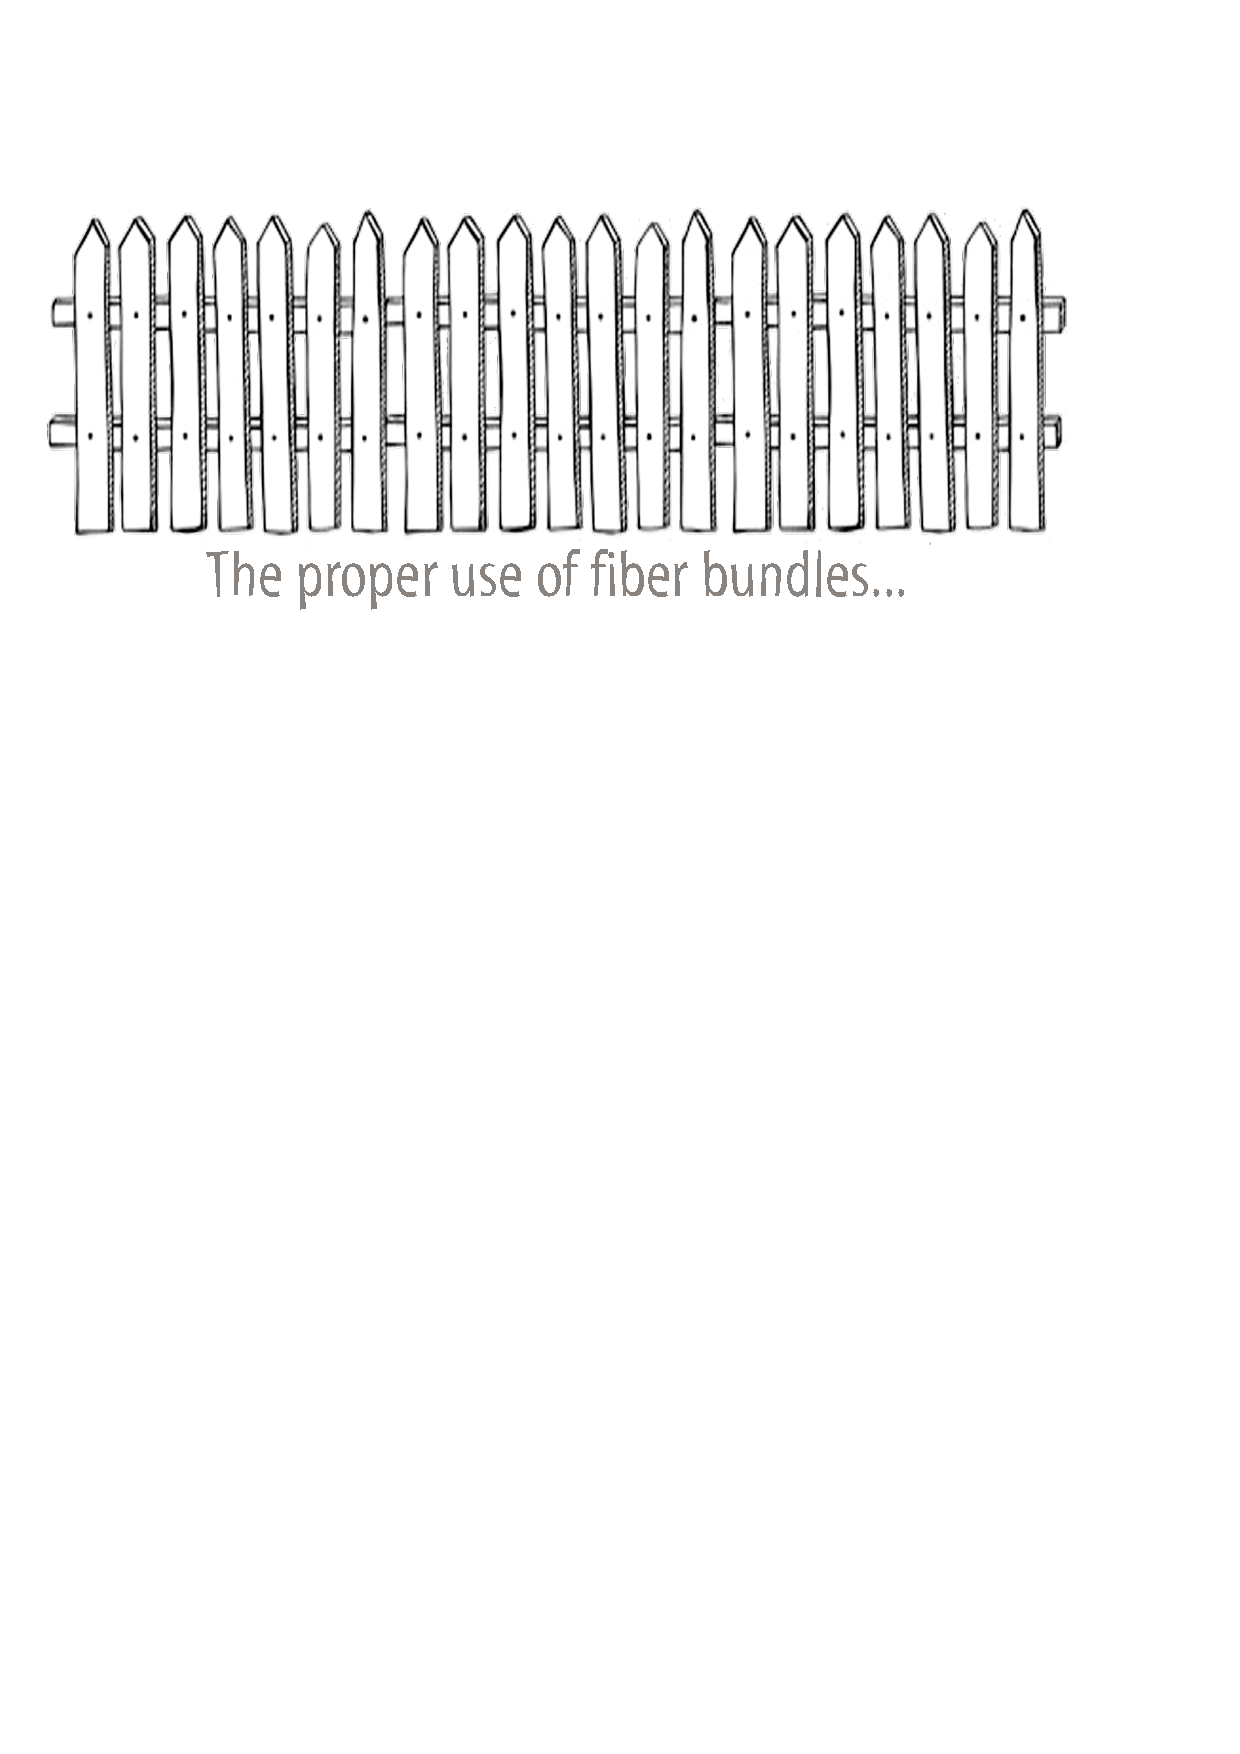
\includegraphics[width=\textwidth]{Figures/Fence.pdf}}
\vfill
